\documentclass[12pt,fleqn]{article}

\usepackage[english]{babel}
\usepackage{SpeedyGonzales}
\usepackage{MediocreMike}
%\usepackage{Blastoise}

\title{
    Project plan:\\
    An Open Source Danish Knowledge Graph Language Model
}


\author{Søren Winkel Holm, Asger Laurits Schultz\\s183911, s183912}
\date{\today}

\pagestyle{fancy}
\fancyhf{}
\lhead{Søren Winkel Holm, Asger Laurits Schultz}
\chead{}
\rhead{Technical University opip f Denmark}
\lfoot{Plan for BSc. project}
\rfoot{Page \thepage{} of \pageref{LastPage}}

\graphicspath{{imgs/}}
\linespread{1.15}

\begin{document}
\maketitle\noindent
Natural Language Processing (NLP) is one of the subfields of Artificial Intelligence with the clearest practical applicability.
It is, however, also one of the most data hungry fields, resulting in a limited success in transferring methods from English to low-resource language domains such as Danish.
A possible mitigation of this limitation of statistical learning is the introduction of explicit knowledge in the modelling, which will be explored in this project.

The contextualized word representation model LUKE (Language Understanding using Knowledge Embeddings) combines explicit knowledge of named entities mined from Wikipedia with deep learning in the form the Transformer architecture. \cite{transformer}
The primary goal of this bachelor project is to produce and analyze daLUKE, a Danish entity-aware model following the LUKE architecture.
The NLP subtask of Named Entity Recognition (NER) will be the main approach to examine the performance of the model.

As a part of the project, we aim to
\begin{itemize}
    \item reproduce existing Danish NER results on a number of public NER datasets and reproduce the NER results of the English LUKE
    \item pre-train a Danish LUKE-based model on the Danish Wikipedia
    \item fine-tune daLUKE on NER and compare its performance and predictions to existing NER models - particularly Danish BERT\footnote{\url{https://github.com/botxo/nordic\_bert}}
    \item optimize the performance of daLUKE, possibly by changes to data and architecture, and perform a open-source release of the pre-trained model
\end{itemize}

\section*{Learning outcomes}%
\begin{enumerate}
    \item Understand and apply a Machine Learning approach that combines explicit knowledge with statistical learning
    \item Apply the training of Deep Natural Language Processing models to a low resource language
    \item Implement an open-source Deep Learning model, allowing easy reproduction and application
    \item Compare and analyze performance of Natural Language Processing models on an entity-related task and discuss their practical use
\end{enumerate}

\begin{figure}[H]
    \centering
        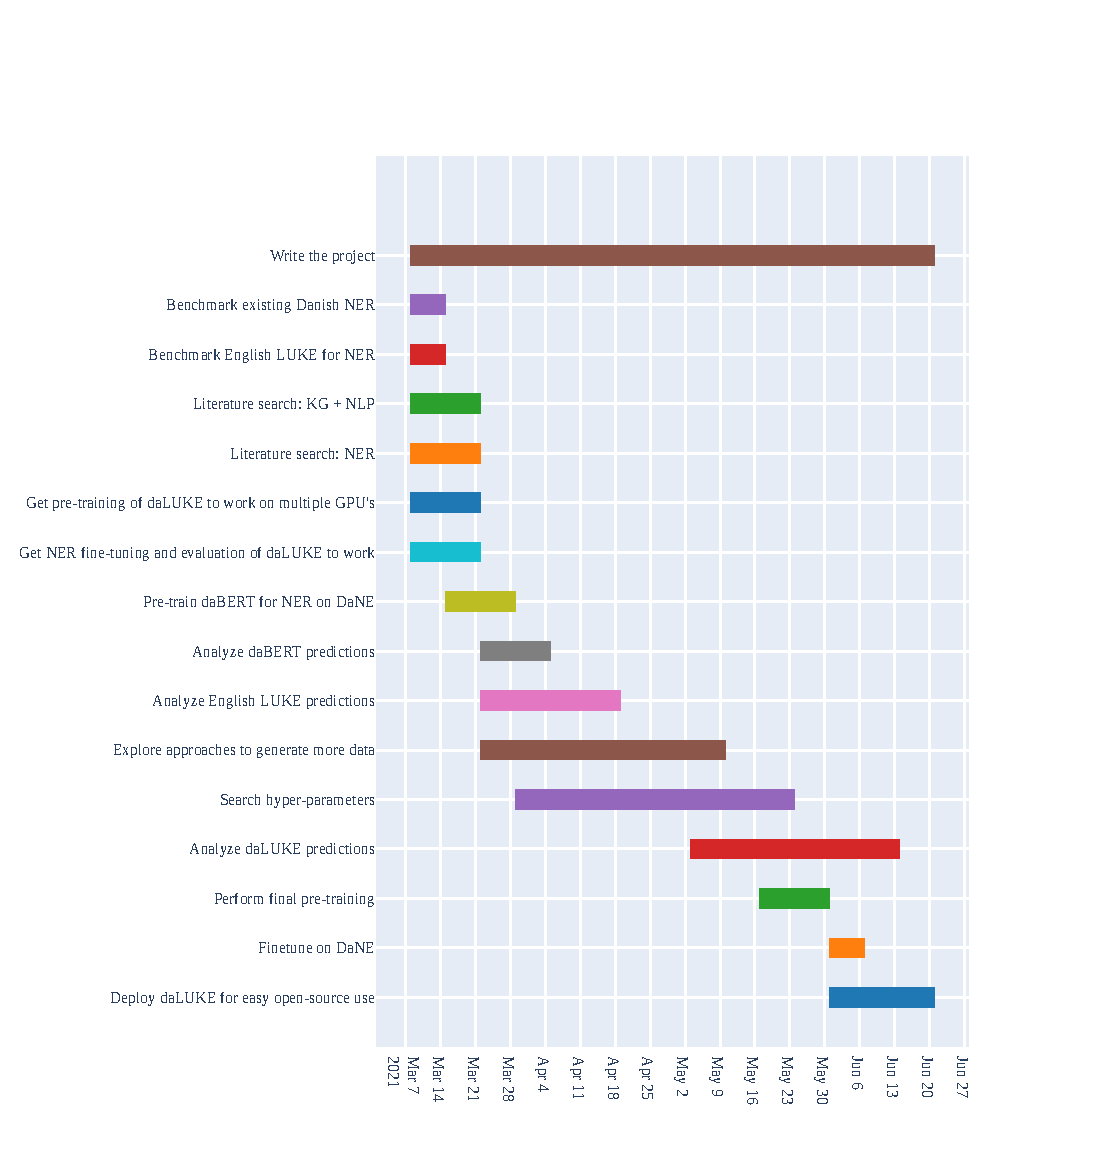
\includegraphics[width=\linewidth]{gantt}
        \caption{Gantt chart showing the current, quite tentative, project timeline}
    \label{fig:gantt}
\end{figure}\noindent

\begin{thebibliography}{9}
    \bibitem{transformer} Vaswani, A. et al.: "Attention is all you need". \url{https://arxiv.org/abs/1706.03762v5}
\end{thebibliography}


\end{document}
